\documentclass[aspectratio=169]{beamer}

\usetheme{metropolis}
\usepackage[T1]{fontenc}
\usepackage{booktabs}
\usepackage{graphicx}
\usepackage{subcaption}
\usepackage{enumitem}

\setlist[itemize]{itemsep=3pt,topsep=2pt,parsep=0pt}

\graphicspath{{../article/plots/}}

\newcommand{\code}[1]{%
  \begingroup
  \renewcommand{\_}{\textunderscore\allowbreak}%
  \texttt{#1}%
  \endgroup
}

\setbeamerfont{title}{size=\Large}

\title{A Graph-based Framework for Coverage Analysis in Autonomous Driving}
\author{Thomas Mühlenstädt \and Marius Bause}
\date{}

\begin{document}

\maketitle

% ---------------------------------------------------------
\begin{frame}{Motivation and Existing Approaches}
\begin{columns}[t]
\begin{column}{0.5\textwidth}
\textbf{Motivation}
\begin{itemize}[itemsep=1pt,topsep=1pt,parsep=0pt]
    \scriptsize
    \item Coverage analysis is crucial to ensure safety and reliability of autonomous driving systems
    \item Coverage argument: have the observed scenes exhausted the space of traffic scenes that can occur?
    \item Existing arguments are typically collected \textbf{per coverage factor}, or up to 2--3 factor interactions
    \item This work: take the \textbf{complete traffic scene} as the unit of coverage
    \begin{itemize}[itemsep=1pt,topsep=1pt,parsep=0pt]
        \item each scene $\rightarrow$ one graph
        \item nodes carry actor parameters, edges carry relation parameters
        \item arbitrarily complex scenes (varying numbers of actors, higher-order interactions) captured in one object, not decomposed into isolated factors
    \end{itemize}
    \item Scope: completeness of observed scenes, \emph{not} safety of the system
\end{itemize}
\end{column}
\begin{column}{0.5\textwidth}
\textbf{Existing Approaches}
\begin{itemize}[itemsep=1pt,topsep=1pt,parsep=0pt]
    \scriptsize
    \item Scenario-based testing is the dominant paradigm (PEGASUS: functional / logical / concrete scenario levels)
    \item \textbf{Approval trap}: statistically demonstrating superior safety needs billions of test km
    \item $\rightarrow$ motivates simulation and systematic coverage methods
    \item Standardized coverage criteria: ISO~21448, UL~4600
    \item Domain-specific coverage buckets (Foretellix)
    \item Recent trend: represent traffic scenes as \textbf{graphs} for scalable, label-free analysis
    \begin{itemize}[itemsep=1pt,topsep=1pt,parsep=0pt]
        \item semantic scene-graph embeddings, contrastive learning, heterogeneous scenario graphs
    \end{itemize}
    \item Gap: these graph representations are not designed specifically for coverage analysis $\rightarrow$ this work
\end{itemize}
\end{column}
\end{columns}
\end{frame}

% ---------------------------------------------------------
\begin{frame}{Datasets}
\begin{itemize}
    \item \textbf{Argoverse 2.0}: large-scale real-world dataset
    \begin{itemize}
        \item 250{,}000 scenarios, 11\,s each
        \item tracked trajectories (vehicles, pedestrians, cyclists) + semantic map
        \item subset of 17{,}000 training scenes used
    \end{itemize}
    \item \textbf{CARLA} 0.9.15: open-source simulator
    \begin{itemize}
        \item six maps, 20--60 vehicles per run, mixed traffic
        \item 2{,}050 scenes of 11\,s each
    \end{itemize}
\end{itemize}
\end{frame}

% ---------------------------------------------------------
\begin{frame}{Traffic Scene Graph and Construction Algorithm}
\begin{columns}[t]
\begin{column}{0.5\textwidth}
\textbf{\footnotesize Defining a Traffic Scene Graph}
\begin{itemize}[itemsep=1pt,topsep=1pt,parsep=0pt]
    \scriptsize
    \item \textbf{Map graph} $G_{\text{map}}$: nodes = lane segments (geometry + semantics)
    \item Map graph edges: \textbf{following}, \textbf{neighbor}, \textbf{opposite}
    \item \textbf{Actor graph} $G_{\text{actor}}$: nodes = actors at one timestep (lane, position, speed, type, lane-change indicator)
    \item Actor graph edges: relation type + path length
    \item Relation types (semantic hierarchy): \textbf{Following/Leading}, \textbf{Neighbor}, \textbf{Opposite}
    \item Lane-change indicator ($\Delta t = 1$\,s) captures cut-in/cut-out within a single-timestep graph
\end{itemize}
\end{column}
\begin{column}{0.5\textwidth}
\textbf{\footnotesize Hierarchical Graph Construction Algorithm}
\begin{itemize}[itemsep=1pt,topsep=1pt,parsep=0pt]
    \scriptsize
    \item \textbf{Phase 1 -- Relation Discovery}: find a connecting path per actor pair; path structure sets relation type; filtered by distance/path-length thresholds
    \item \textbf{Phase 2 -- Hierarchical Construction}: add edges leading/following $\rightarrow$ neighbor $\rightarrow$ opposite (shortest path first); skip an edge if a path already exists (BFS)
\end{itemize}
\begin{table}
\centering
\tiny
\begin{tabular}{lcc}
\toprule
\textbf{Relation} & \textbf{Dist.\ fwd/bwd [m]} & \textbf{Max.\ path [edges]} \\
\midrule
Leading/following & 100 & 3 \\
Neighbor          & 50 / 50 & 2 \\
Opposite          & 100 / 10 & 2 \\
\bottomrule
\end{tabular}
\end{table}
\end{column}
\end{columns}
\end{frame}

% ---------------------------------------------------------
\begin{frame}{Hierarchical Construction: Example}
\begin{columns}
\begin{column}{0.48\textwidth}
    \centering
    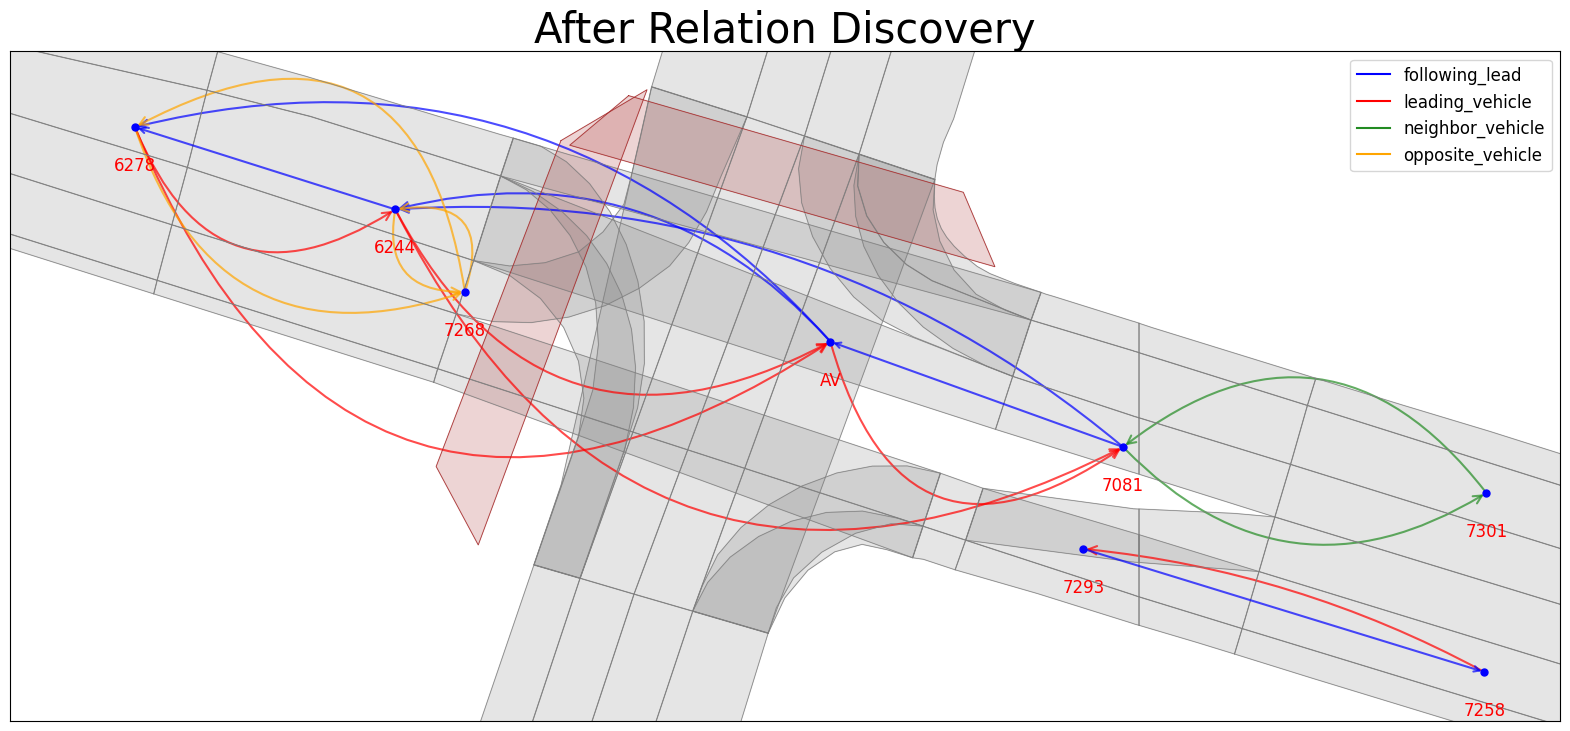
\includegraphics[width=\textwidth]{graph_construction/5758074f-be16-49da-8bb5-d43a0d8cd034_after_discovery.png}
    \\ \footnotesize After relation discovery
\end{column}
\begin{column}{0.48\textwidth}
    \centering
    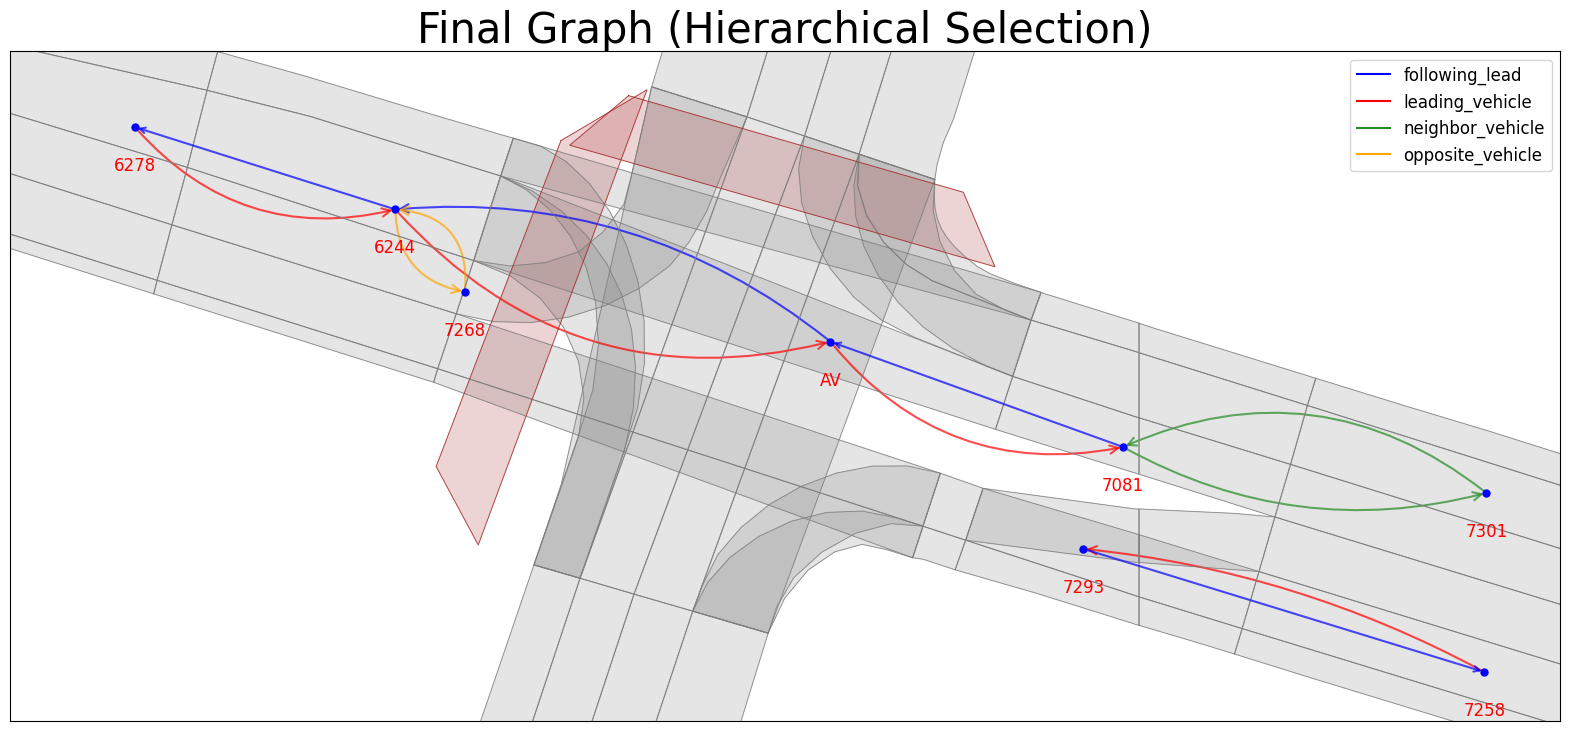
\includegraphics[width=\textwidth]{graph_construction/5758074f-be16-49da-8bb5-d43a0d8cd034_final.png}
    \\ \footnotesize After hierarchical selection
\end{column}
\end{columns}
\vspace{0.5em}
\small The discovery graph (left) contains all relations within distance limits. Hierarchical selection (right) removes redundant edges representable through existing paths.
\end{frame}

% ---------------------------------------------------------
\begin{frame}{Coverage Method 1: Subgraph Isomorphism}
\begin{itemize}[itemsep=2pt,topsep=2pt,parsep=0pt]
    \small
    \item Traffic scene archetypes (lead-follow, cut-in, cut-out, opposite traffic, platoons, \dots) expressed as small graphs
    \item Check whether a subgraph of scene graph $G$ is isomorphic to archetype $A$ (VF2 algorithm)
    \item Strategy:
    \begin{itemize}[itemsep=1pt,topsep=1pt,parsep=0pt]
        \item define archetype set $S$
        \item fix node/edge attributes considered
        \item match each scene graph against $S$ $\rightarrow$ coverage table $C$
    \end{itemize}
    \item \textbf{18 archetypes} defined: 2-actor (3), 3-actor (9), 4-actor (4), 5-actor (2)
    \item Archetypes are user-defined, illustrative---not a complete or safety-certified taxonomy
    \item Real safety case: archetypes derived top-down (HARA / UL~4600), completeness of the set is critical
\end{itemize}
\end{frame}

% ---------------------------------------------------------
\begin{frame}{Results: Scenario Archetype Coverage Gaps}
\centering
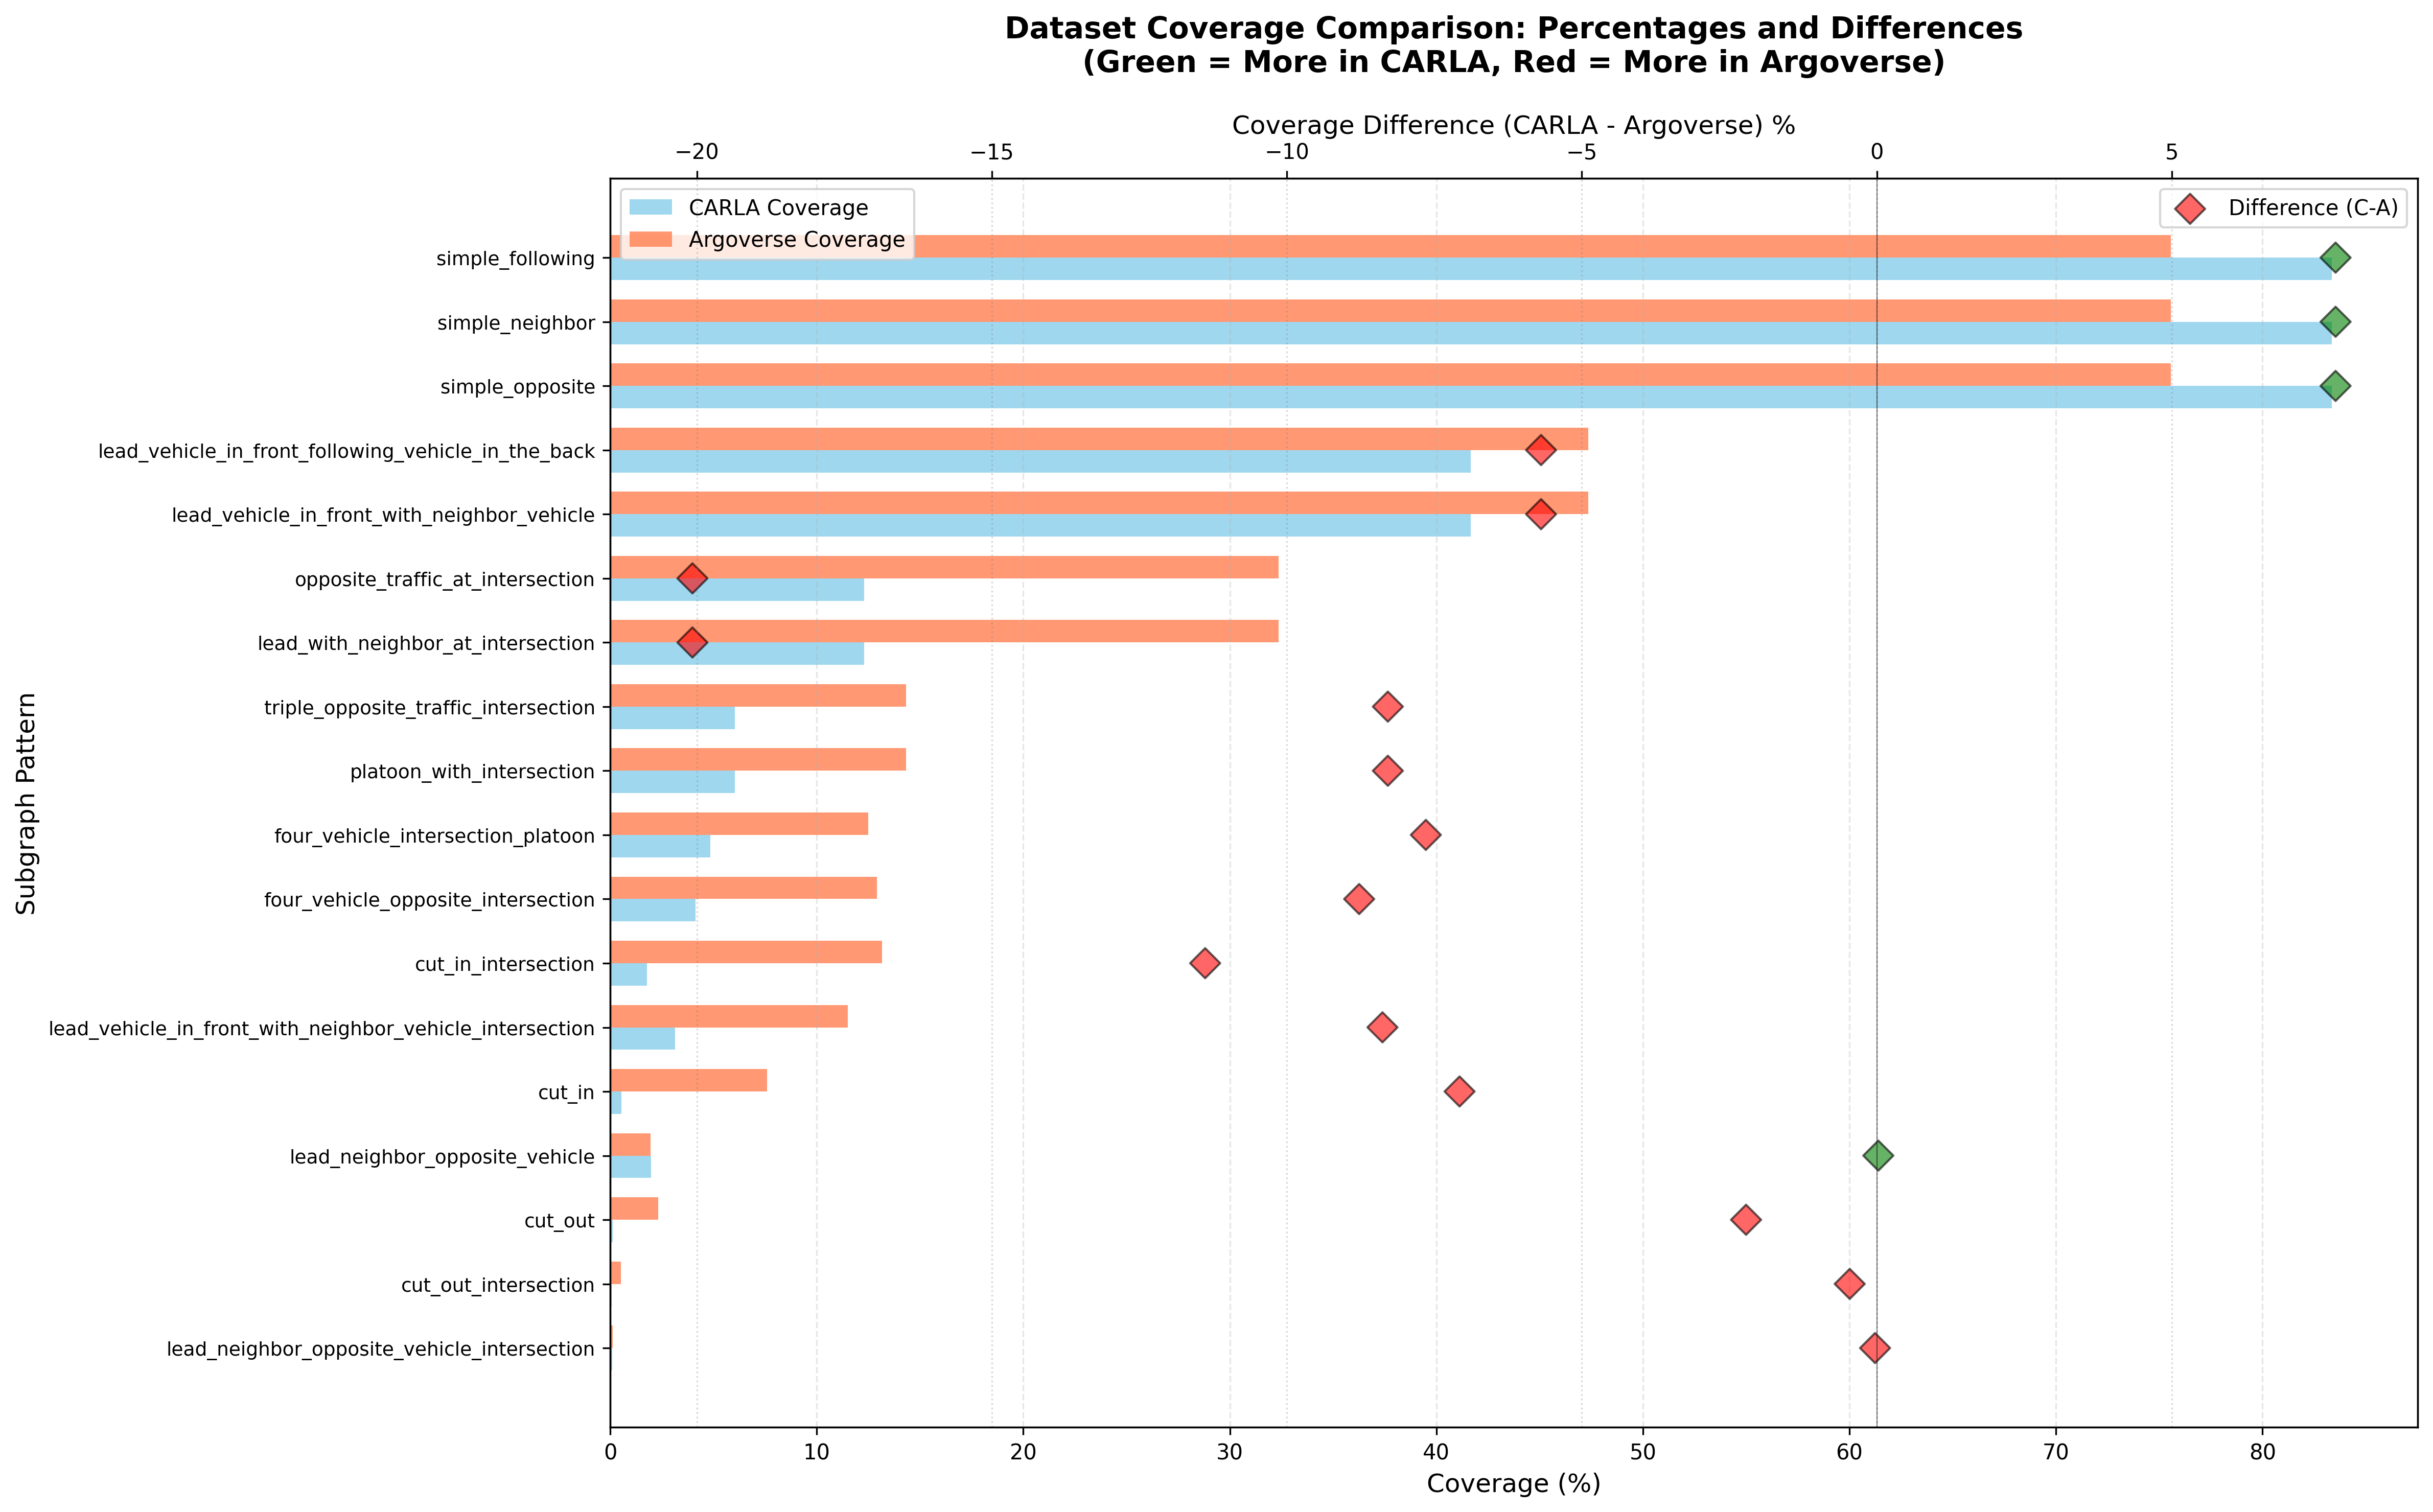
\includegraphics[width=0.42\textwidth]{coverage_comparison_dual_axis.png}
\begin{itemize}
    \footnotesize
    \item CARLA higher coverage only for the 3 simple 2-actor scenarios
    \item All multi-actor scenarios: Argoverse shows higher occurrence
    \item \code{cut\_out\_intersection}: $<$1\% CARLA vs.\ $\sim$8\% Argoverse
    \item \code{lead\_neighbor\_opposite\_vehicle\_intersection}: $\sim$6\% Argoverse, virtually absent in CARLA
    \item \code{cut\_in}/\code{cut\_out}: underrepresented in CARLA regardless of intersections
\end{itemize}
\end{frame}

% ---------------------------------------------------------
\begin{frame}{Results: Parameter Distribution Gaps}
\begin{columns}
\begin{column}{0.55\textwidth}
    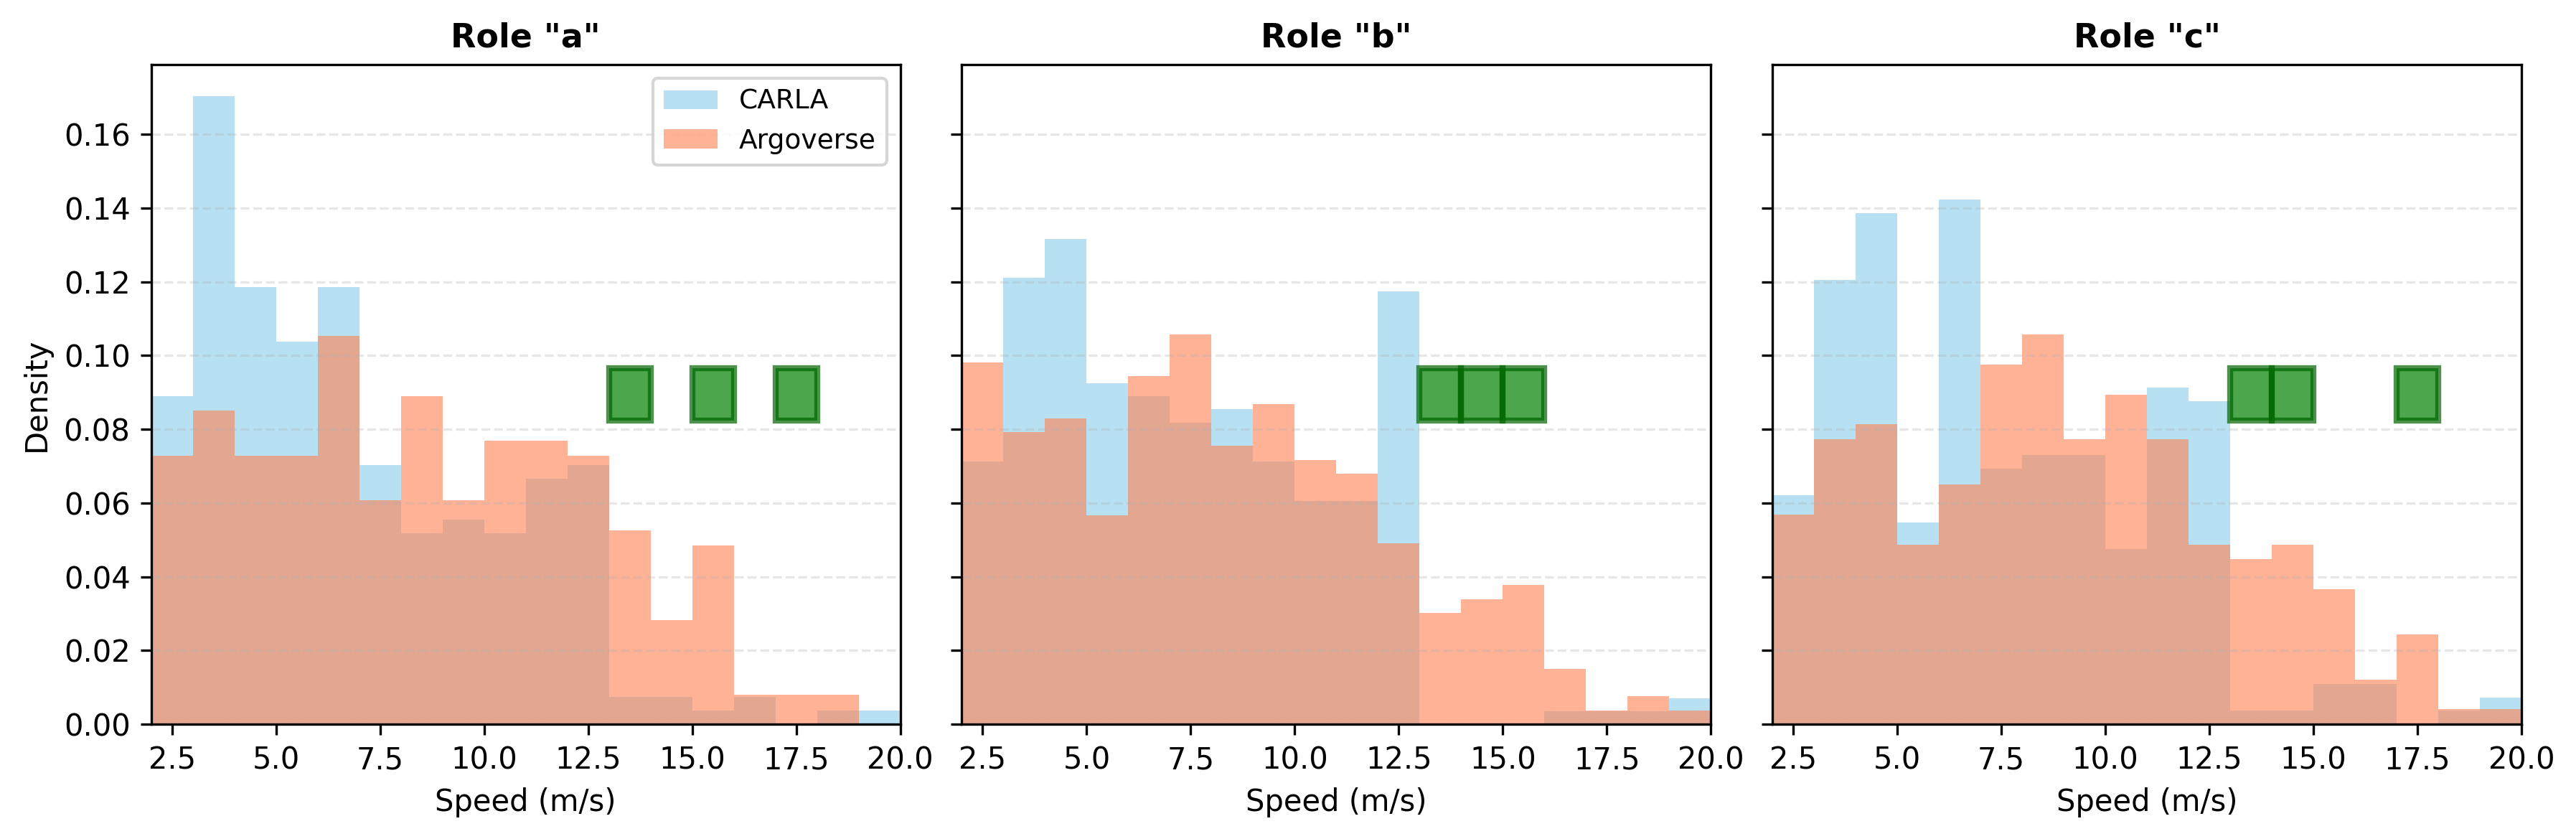
\includegraphics[width=\textwidth]{role_comparison_lead_vehicle_in_front_with_neighbor_vehicle.png}
\end{column}
\begin{column}{0.45\textwidth}
    \small
    \begin{itemize}
        \item Role-specific speed distributions, \code{lead\_vehicle\_in\_front\_with\_neighbor\_vehicle} scenario
        \item CARLA concentrates around 3--5\,m/s
        \item Argoverse extends to 15--20\,m/s and beyond
        \item Coverage gap in the 13--17\,m/s range for all three roles
        \item Gaps arise at the parameter level even within structurally matching scenarios
    \end{itemize}
\end{column}
\end{columns}
\end{frame}

% ---------------------------------------------------------
\begin{frame}{Coverage Method 2: Graph Embeddings (GINE)}
\begin{itemize}
    \item Real traffic scenes are far more complex than predefined archetypes $\rightarrow$ complementary top-down approach
    \item Graph Isomorphism Network with Edge features (GINE): natively encodes edge attributes (relation type + distance)
    \item Self-supervised contrastive training (NT-Xent/InfoNCE, $\tau=0.07$) on CARLA + Argoverse jointly
\end{itemize}
\centering
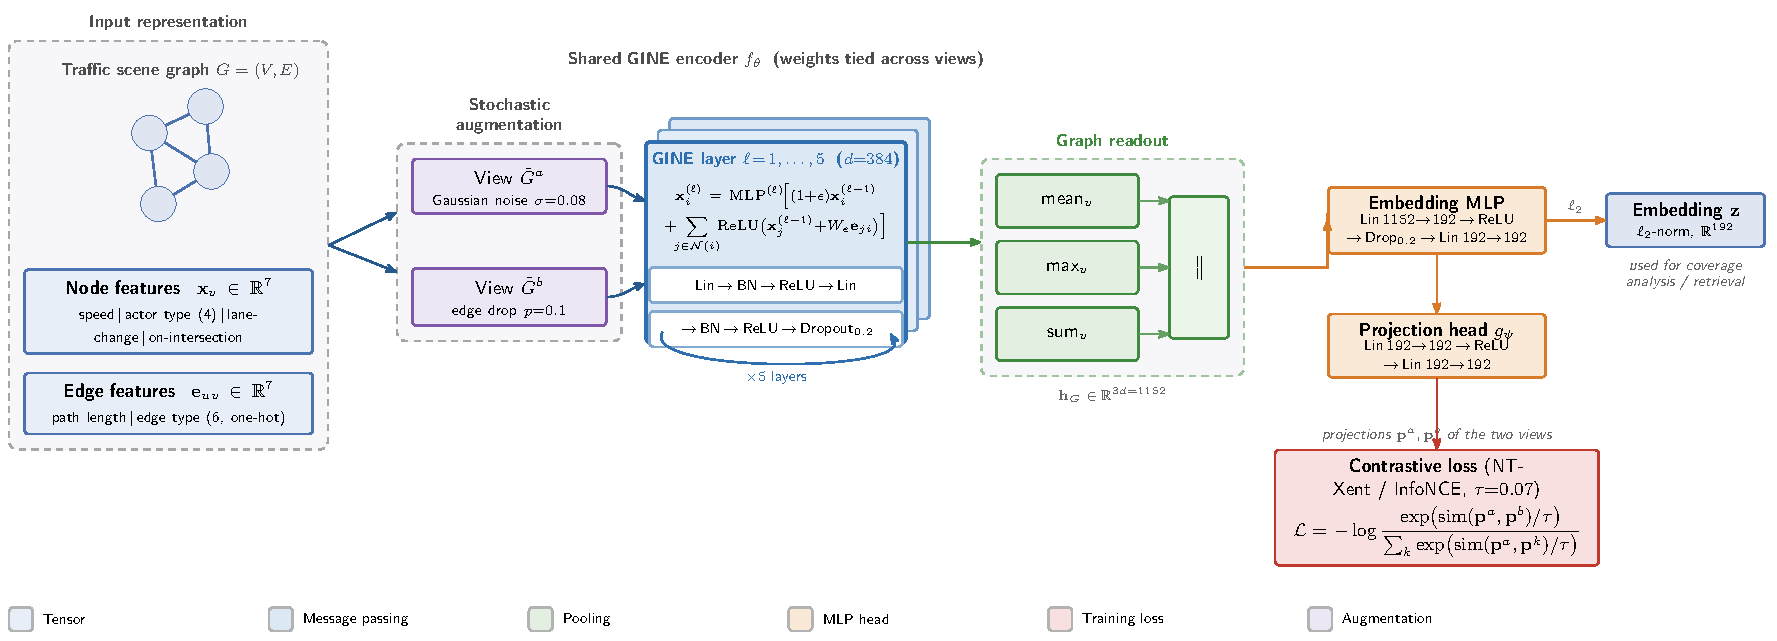
\includegraphics[width=0.8\textwidth]{graph_gine_architecture_tikz.pdf}
\end{frame}

% ---------------------------------------------------------
\begin{frame}{Results: Embedding Space Analysis}
\begin{columns}
\begin{column}{0.5\textwidth}
    \centering
    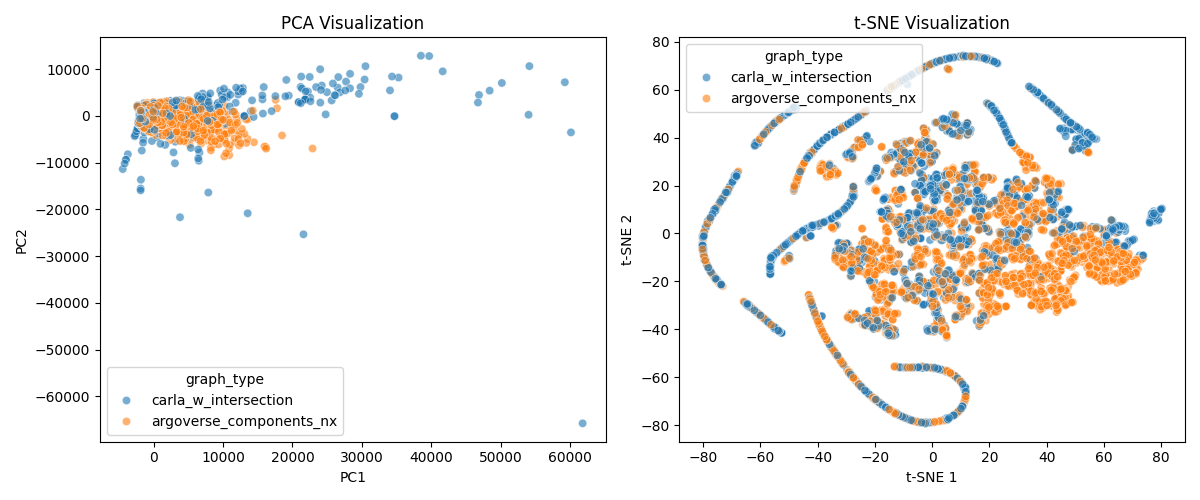
\includegraphics[width=\textwidth]{graph_embeddings_pca_tsne_test_plot.png}
\end{column}
\begin{column}{0.5\textwidth}
    \centering
    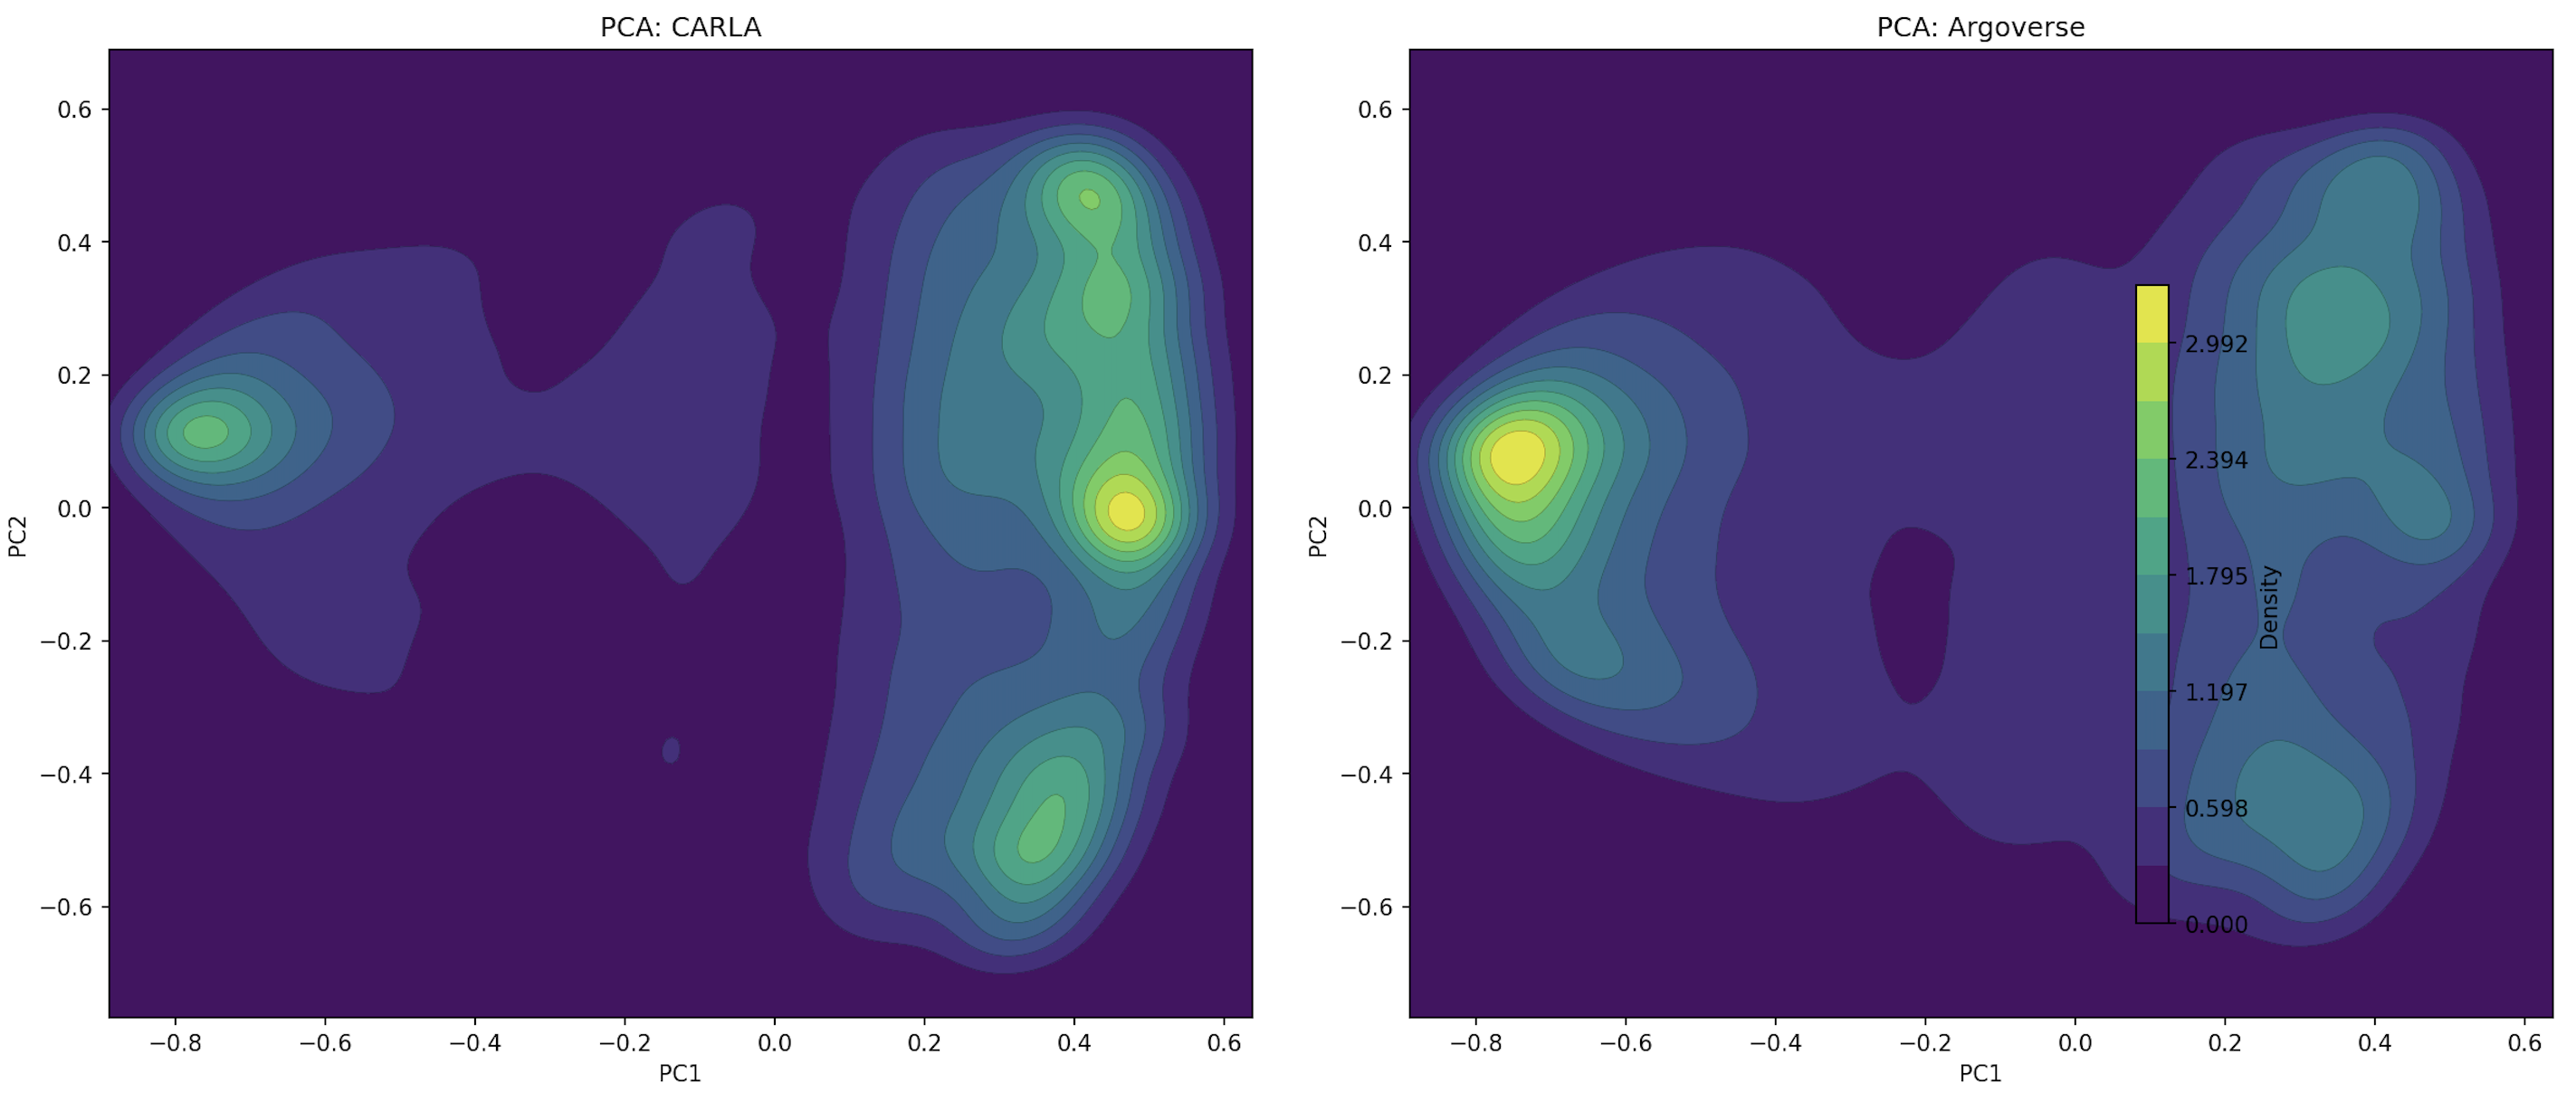
\includegraphics[width=\textwidth]{PCA_density_plots_manually_cropped.png}
\end{column}
\end{columns}
\vspace{0.5em}
\small
\begin{itemize}
    \item Plausibility check: nearest neighbours in embedding space share actor configuration and road geometry
    \item First two principal components explain 40\% of the total variance
    \item CARLA peaks at higher PC1 values
    \item Argoverse peaks at negative PC1 values
    \item $\rightarrow$ datasets occupy different regions of the embedding space
\end{itemize}
\end{frame}

% ---------------------------------------------------------
\begin{frame}{Results: Coverage Gaps in Embedding Space}
\centering
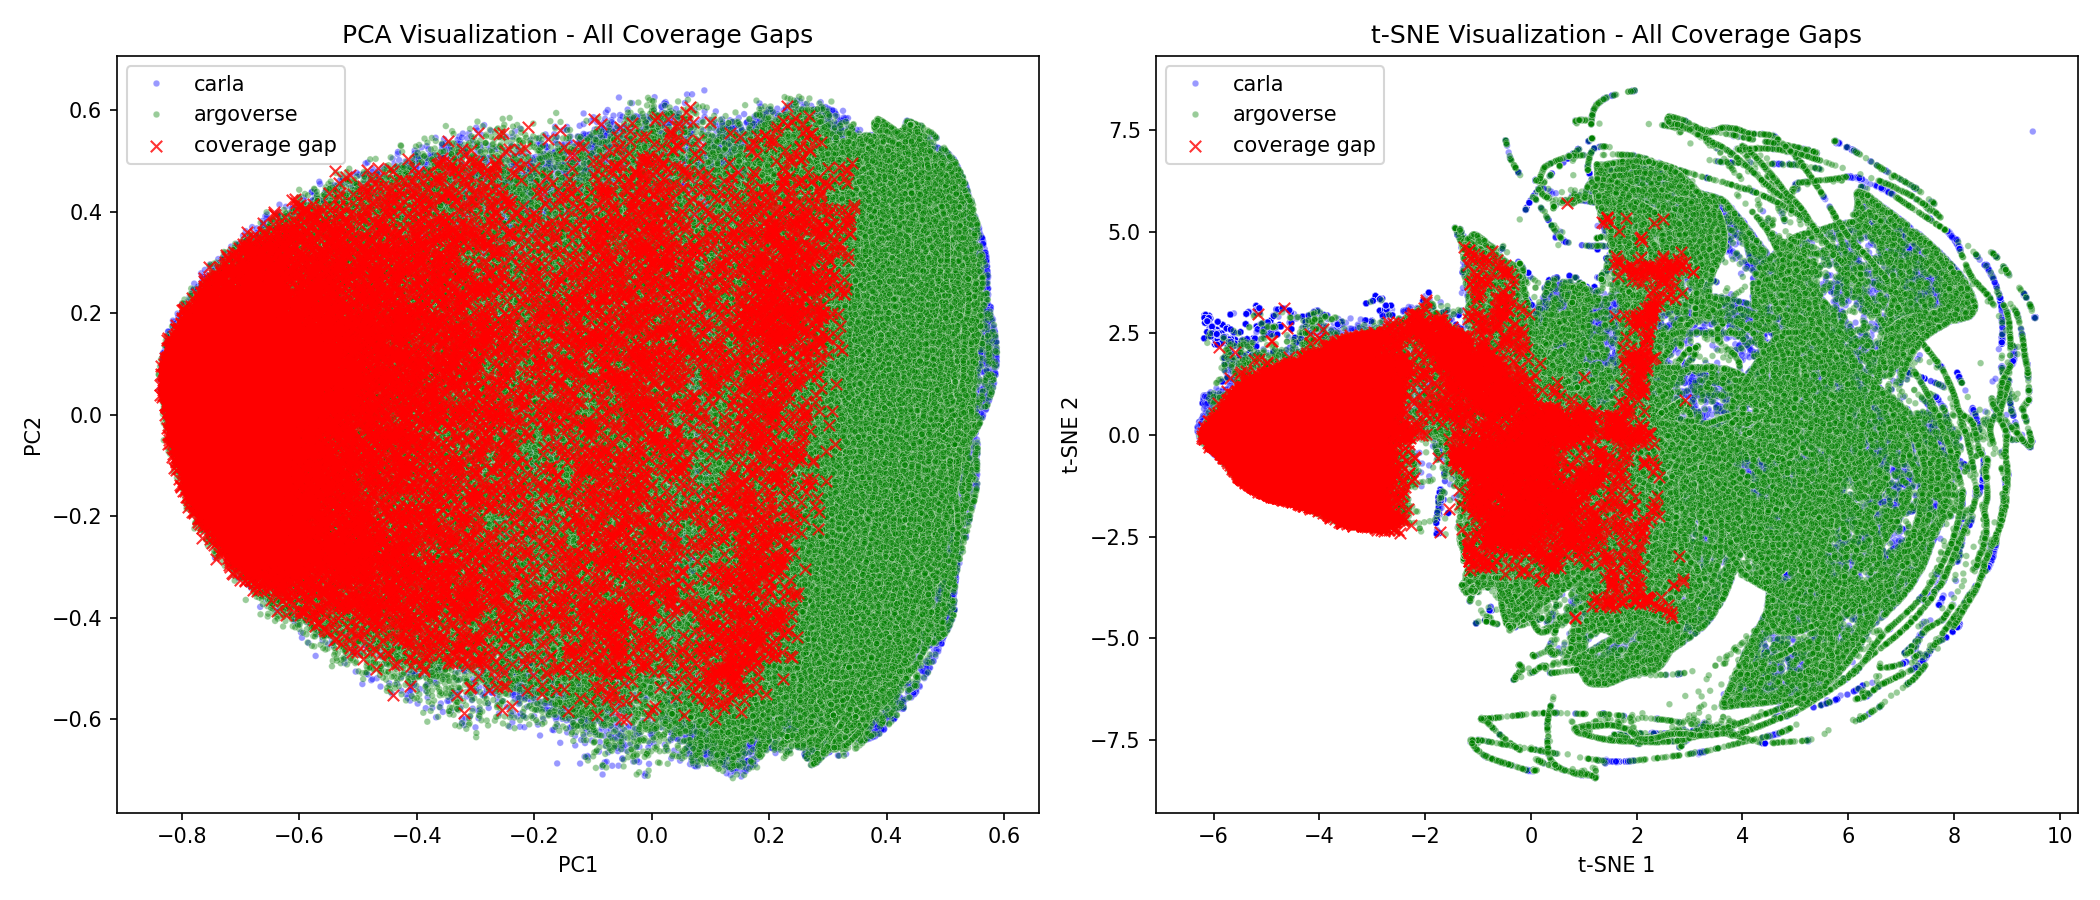
\includegraphics[width=0.5\textwidth]{graph_embeddings_coverage_gap_visualization.png}
\begin{itemize}
    \footnotesize
    \item Argoverse graphs with under-represented archetype labels projected into embedding space and compared against CARLA density
    \item \textbf{23{,}148} Argoverse graphs identified as coverage gaps
    \item Dominated by \code{cut\_in} ($\sim$94\% of Argoverse cut-in instances), \code{cut\_out}, \code{cut\_out\_intersection}, \code{lead\_neighbor\_opposite\_vehicle\_intersection}
    \item Gap graphs cluster where CARLA density is negligible $\rightarrow$ agreement between embedding and exact isomorphism labels
    \item Used as a coverage-\emph{screening} layer, not a standalone safety oracle
\end{itemize}
\end{frame}

% ---------------------------------------------------------
\begin{frame}{Summary and Future Work}
\begin{itemize}
    \footnotesize
    \item Graph-based framework: hierarchical scene graphs combining map topology with actor relationships
    \item Two complementary coverage methods:
    \begin{itemize}
        \item subgraph isomorphism against archetypes $\rightarrow$ interpretable, pattern-based coverage
        \item GINE embeddings via contrastive learning $\rightarrow$ similarity-based coverage, clustering, anomaly detection
    \end{itemize}
    \item Validated on Argoverse 2.0 and CARLA: reveals structural, parametric, and co-occurrence coverage gaps in simulation
    \item Scales across scenarios without scenario-specific handling
    \item Naturally accommodates varying numbers of actors
    \item \textbf{Future work}:
    \begin{itemize}
        \item multi-timestep temporal graphs
        \item automatically extracting new archetype candidates from dense, unmatched embedding regions
    \end{itemize}
    \item Code: \url{https://github.com/tmuehlen80/graph_coverage}
\end{itemize}
\end{frame}

\end{document}
